\documentclass{article}

\usepackage[utf8]{inputenc}
\usepackage[dvipsnames]{xcolor}
\usepackage{multirow}
\usepackage{array}
\usepackage{float}
\usepackage{graphicx}
\usepackage[caption=false]{subfig}
\usepackage{hyperref}
\usepackage{amsmath}
%\usepackage[backend=biber,style=numeric,sorting=none]{biblat‌​ex}

\title{Building a sequence aligner capable of affine gap penalties.}
\date{October 2018}
\author{Isak Johansson-\AA{}khe, Linköping University}

\begin{document}
\maketitle

\section*{Introduction}
Protein-protein sequence alignment is the basis and first step of many bioinformatical methods. In 1970, the first draft of the Needleman-Wunsch algorithm for global sequence alignment was first introduced \cite{needleman1970general}. This was a simple algorithm, with no gap penalties (only rewards or penalties for matches or mismatches), and cubic complexity. Through the years, many great additions have come to this first basis for sequence alignment, including gap penalties, \textit{affine gap penalties}, a simplification to quadratic complexity, and the option for finding the best local alignments with the Smith-Waterman algorithm \cite{smith1981comparison}.

In this short project, an aligner capable of finding both global and local alignments while using the affine gap penalty is implemented and briefly analyzed.

\section*{Theory}
Presented below are the respective algorithms for global and local alignment using affine gap penalties.
\subsection*{Needleman-Wunsch with Affine Gap Penalty}
\subsubsection*{Input:}
Sequences $A$ and $B$ to be aligned.

\subsubsection*{Variables:}
\indent\indent
$i \in \{1, 2, ..., n\}$

$j \in \{1, 2, ..., m\}$

$M(i,j)$

$G_{x}(i,j)$

$G_{y}(i,j)$

where $n$ and $m$ are the lengths of sequences $A$ and $B$, respectively.

\subsubsection*{Initialization:}
\indent\indent
$M(0,0) = 0$

$G_{x}(i,0) = h + g \times i$

$G_{y}(0,j) = h + g \times j$

all other cells: $-\infty$

where $h$ is the penalty for opening a new gap and $g$ is the penalty for extending a gap.

\subsubsection*{Calculations:}

For all $i$ and $j$, do:

\begin{equation}
M(i,j) = \max 
	\begin{cases}
		M(i-1,j-1) + s(x_{i}, y_{j}),\\
		G{x}(i-1,j-1) + s(x_{i}, y_{j}),\\
		G_{y}(i-1,j-1) + s(x_{i}, y_{j})\\
	\end{cases}
\end{equation}
\begin{equation}
G_{x}(i,j) = \max
	\begin{cases}
		M(i-1,j) + h + g, \\
		G_{x}(i-1,j) + g\\
	\end{cases}
\end{equation}
\begin{equation}
G_{y}(i,j) = \max
	\begin{cases}
		M(i,j-1) + h + g, \\
		G_{y}(i,j-1) + g\\
	\end{cases}
\end{equation}
where $s$ is the scoring matrix used, $x_{i}$ is the amino acid at position $i$ in sequence $A$, and $y_{j}$ is the amino acid at position $j$ in sequence $B$.

\subsubsection*{Traceback}
Start at $\max(M(n,m), G_{x}(n,m), G_y{n,m})$ and follow pointers back to $M(0,0)$, $G_{x}(0,0)$, or $G_y{0,0}$, introducing gaps in A and B when moving in $G_{x}$ or $G_{y}$ respectively, and matches when moving in $M$.

\subsection*{Smith-Waterman with Affine Gap Penalty}
\subsubsection*{Input:}
Sequences $A$ and $B$ to be aligned.

\subsubsection*{Variables:}
\indent\indent
$i \in \{1, 2, ..., n\}$

$j \in \{1, 2, ..., m\}$

$M(i,j)$

$G_{x}(i,j)$

$G_{y}(i,j)$

where $n$ and $m$ are the lengths of sequences $A$ and $B$, respectively.

\subsubsection*{Initialization:}
\indent\indent
$M(0,0) = 0$

$G_{x}(i,0) = \max(h + g \times i, 0)$

$G_{y}(0,j) = \max(h + g \times j, 0)$

all other cells: $-\infty$

where $h$ is the penalty for opening a new gap and $g$ is the penalty for extending a gap.

\subsubsection*{Calculations:}

For all $i$ and $j$, do:

\begin{equation}
M(i,j) = \max 
\begin{cases}
M(i-1,j-1) + s(x_{i}, y_{j}),\\
G_{x}(i-1,j-1) + s(x_{i}, y_{j}),\\
G_{y}(i-1,j-1) + s(x_{i}, y_{j}),\\
0\\
\end{cases}
\end{equation}
\begin{equation}
G_{x}(i,j) = \max
\begin{cases}
M(i-1,j) + h + g, \\
G_{x}(i-1,j) + g\\
\end{cases}
\end{equation}
\begin{equation}
G_{y}(i,j) = \max
\begin{cases}
M(i,j-1) + h + g, \\
G_{y}(i,j-1) + g\\
\end{cases}
\end{equation}
where $s$ is the scoring matrix used, $x_{i}$ is the amino acid at position $i$ in sequence $A$, and $y_{j}$ is the amino acid at position $j$ in sequence $B$.

\subsubsection*{Traceback}
Start at largest $M(i,j)$ and follow pointers back to any of $M(0,0) = 0$, introducing gaps in A and B when moving in $G_{x}$ or $G_{y}$ respectively, and matches when moving in $M$.

\subsection*{EMBOSS Implementation}
Commonly available implementations of these algorithms are available via the EMBOSS software package \cite{EMBOSS}. The EMBOSS implementation follow slightly different rules however;
\begin{itemize}
	\item When opening a gap, there is no gap extension penalty added to the first gap.
	\item In the cases that a sequence starts with or ends in a gap, no gap opening penalty is added to the starting and/or ending gap.
\end{itemize}

\section*{Method}
Both Needleman-Wunsch and Smith-Waterman with affine gap penalties were included in the final script created. Additionally, for ease of comparison, an option was included to run the script with the EMBOSS scoring method. This script was called \textit{aligner.py}.

Some light analysis of time efficiency and method complexity was performed, optimizing the script further. Details can be found in the \textit{Project\_supplementary.ipynb} jupyter notebook. The optimized script is called \textit{aligner\_optimized.py}. Both instances of the script was kept separately for ease of comparison.

\section*{Results}
The resulting aligner is complexity $O(nm)$, as derived from tests in \textit{Project\_supplementary.ipynb}, and can manage many different kinds of alignments, as described by its help statement:
\begin{verbatim}
usage: aligner_optimized.py [-h] [-g GAP] [-o OPENGAP] [-e] [-l]
[-m MATRIX] [-c CHARBREAK]
A B

Aligns sequence A and sequence B using affine gap penalties. If
you want to align with regular gap penalties, set the --opengap
flag to 0.

positional arguments:
A                     Sequence A
B                     Sequence B

optional arguments:
-h, --help            show this help message and exit
-g GAP, --gap GAP     Gap extension penalty (should most often
be a negative number).
-o OPENGAP, --opengap OPENGAP
Gap opening penalty (should most often be a negative
number).
-e, --emboss          Use EMBOSS rules for alignment, meaning you
don't receive gap extension when opening a gap, and having
gaps at the end or beginning of a sequence does not
count as opening a gap.
-l, --local           Make a local alignment rather than a global.
-m MATRIX, --matrix MATRIX
Which scoring matrix to use. The matrix should be
saved as a python dictionary in plain-text. Default
behaviour is using the inbuilt PAM250.
-c CHARBREAK, --charbreak CHARBREAK
How many characters per row you want the output to
have. Default is no linebreaks.
\end{verbatim}

A quick analysis of the runtime over aligning randomized sequences of varying length support the complexity prediction, as seen in figure \ref{fig:length_vs_time}.

\begin{figure}[h]
	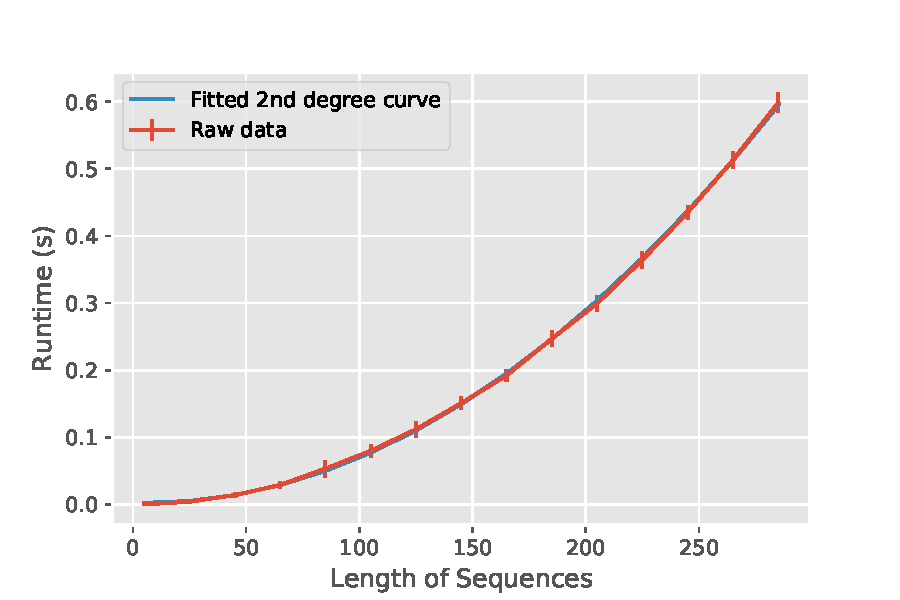
\includegraphics[width=\columnwidth]{timefig}
	\caption{The time for the aligner to finish plotted against the length of the sequences it's tasked to align. All measurements were made with PAM250 matrix, global alignment, open gap penalty of -5, extend gap penalty of -1, and EMBOSS mode turned off. The times are means over 100 random sequences, with the bars showing standard deviation.}
	\label{fig:length_vs_time}
\end{figure}

\section*{Future Work}
The current implementation is in Python, and while this makes it easy to modify and read, this also makes it slow. If this implementation should have any real value, it would have to be reimplemented in a compiled language, such as C.

\bibliographystyle{unsrt}
\bibliography{references}

\end{document}